\documentclass[titlepage,landscape]{seminar}
\usepackage{url}
\usepackage{graphicx}
\usepackage[pdftex]{color}
\usepackage{hyperref}
\usepackage{epstopdf}
\usepackage{slides}

\begin{document}

\myslide{
\[
\pi = \sum x_ix_j\delta_{ij}/N \quad .
\]
\vfill
\begin{eqnarray*}
\E(\pi) &=& \theta \\
\E(k) &=& \theta\sum_i^{n-1} \frac{1}{i} \quad ,
\end{eqnarray*}
\begin{eqnarray*}
\hat \theta_\pi &=& \hat \pi \\
\hat \theta_k   &=& \frac{k}{\sum_i^{n-1}\frac{1}{i}} \quad ,
\end{eqnarray*}
\vfill
\[
\hat D = \hat\theta_\pi - \hat\theta_k 
\]
}

\myslide{
\begin{eqnarray*}
S &=& \mbox{Probability of fewer alleles given observed diversity} \\
F_S &=& \ln\left(\frac{\hat S}{1 - \hat S}\right)
\end{eqnarray*}
}

\myslide{
\[
\mbox{E}(\xi_i) = \frac{\theta}{i} \quad .
\]
\begin{eqnarray*}
\hat\theta_\pi &=& {n \choose 2}^{-1}\sum_{i=1}^{n-1}i(n-i)\hat\xi_i \\
\hat\theta_k  &=& \frac{1}{a_n}\sum_{i=1}^{n-1}\hat\xi_i \\
&& \\
\theta_H &=& {n \choose 2}^{-1}\sum_{i=1}^{n-1}i^2\hat\xi_i \\
\theta_L &=& \frac{1}{n-1}\sum_{i=1}^{n-1}i\hat\xi_i
\end{eqnarray*}
}

\myslide{
\vfill
\begin{eqnarray*}
\theta_H &=& {n \choose 2}^{-1}\sum_{i=1}^{n-1}i^2\hat\xi_i \\
\theta_L &=& \frac{1}{n-1}\sum_{i=1}^{n-1}i\hat\xi_i \\
&& \\
H &=& \hat\theta_\pi - \theta_H  \\
E &=& \theta_L - \theta_k 
\end{eqnarray*}
}

\myslide{
\begin{eqnarray*}
x_{ik} &=& \mbox{frequency of haplotype $i$ in population $k$} \\
x_{i\cdot} &=& \frac{1}{K}\sum_{k=1}^K x_{ik}
\end{eqnarray*}
\vfil
\begin{eqnarray*}
\pi_t &=& \sum_{ij} x_{i\cdot}x_{j\cdot} \delta_{ij} \\
\pi_s &=& \frac{1}{K}\sum_{k=1}^K\sum_{ij} x_{ik}x_{jk}\delta_{ij}
\end{eqnarray*}
\vfil
\[
\Phi_{st} = \frac{\pi_t - \pi_s}{\pi_t}
\]
}

\myslide{
\[
F_{IT} = 1 - \frac{H_i}{H_t} \quad ,
\]
\vfil
\begin{eqnarray*}
1 - F_{IT} &=& (1 - F_{IS})(1 - F_{ST}) \\
1-F_{ST} &=& \frac{1-F_{IT}}{1-F_{IS}} \\
F_{ST} &=&
\frac{\left(1-F_{IS}\right)-\left(1-F_{IT}\right)}{1-F_{IS}} \\
&=& \frac{\left(H_i/H_s\right) - \left(H_i/H_t\right)}{H_i/H_s} \\
&=& 1 - \frac{H_s}{H_t} \\
&=& \frac{H_t - H_s}{H_t}
\end{eqnarray*}
}

\myslide{
\begin{center}
\resizebox{0.75\textwidth}{!}{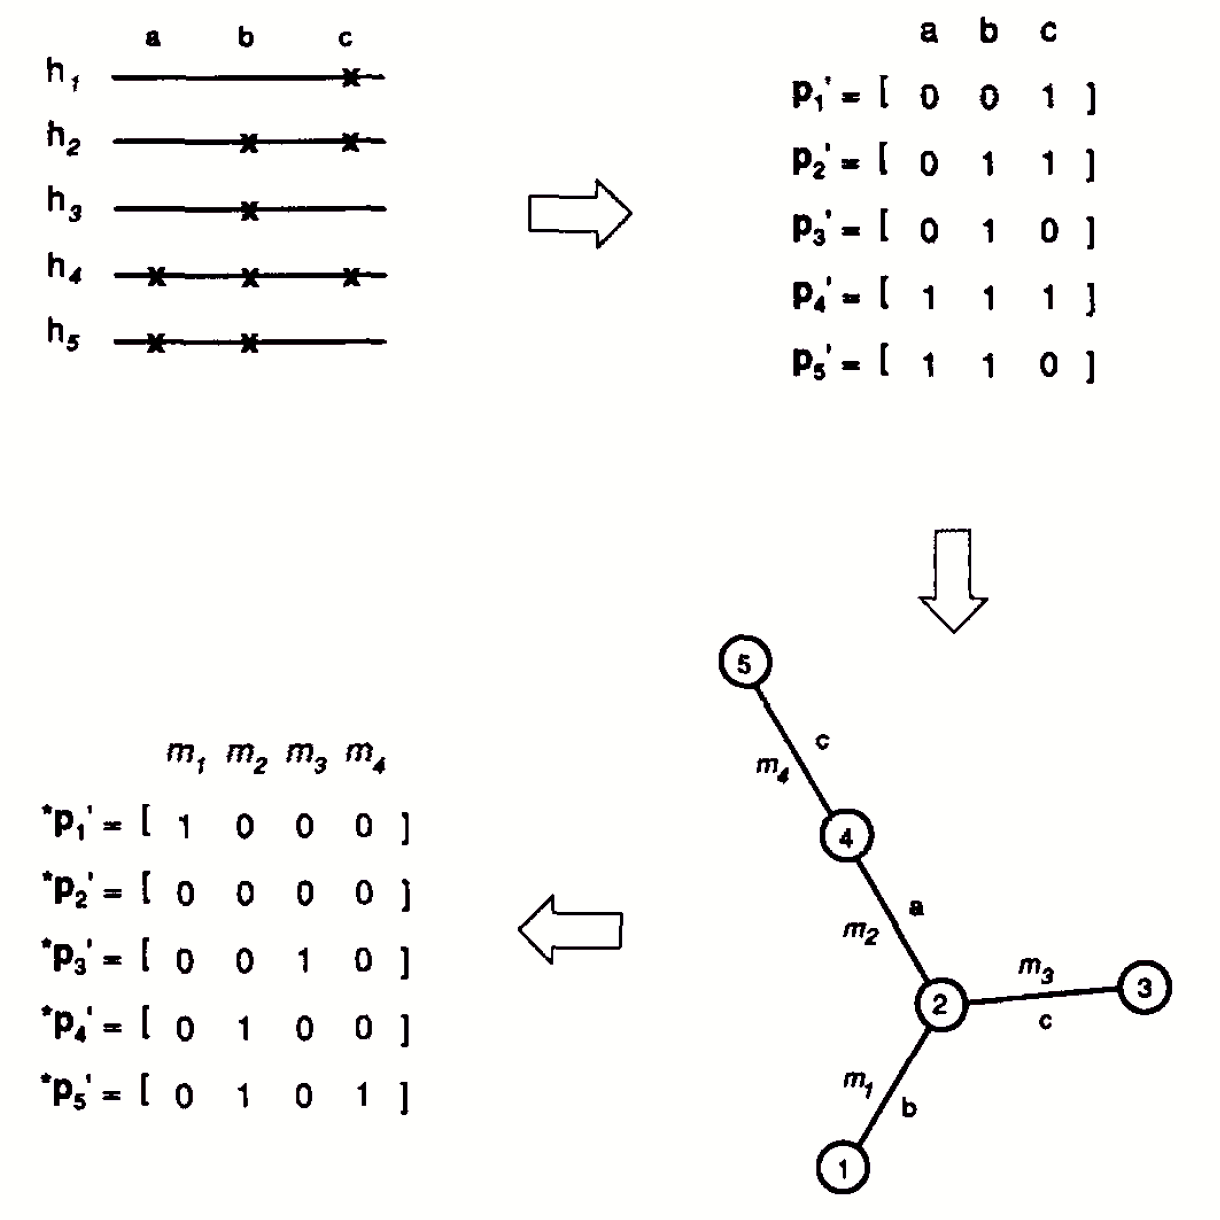
\includegraphics{amova-procedure.eps}}
\end{center}
}

\myslide{
\begin{center}
\resizebox{0.75\textwidth}{!}{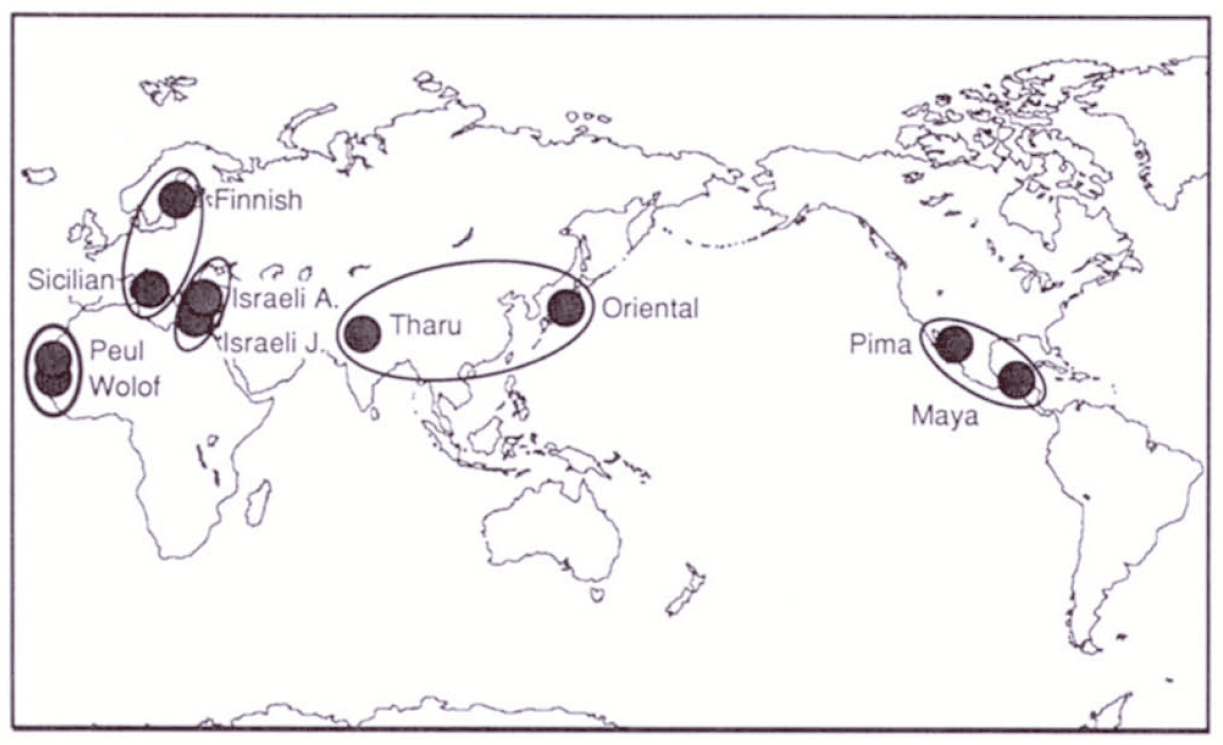
\includegraphics{amova-sample-locations.eps}}
\end{center}
}

\myslide{
\begin{center}
\resizebox{0.75\textwidth}{!}{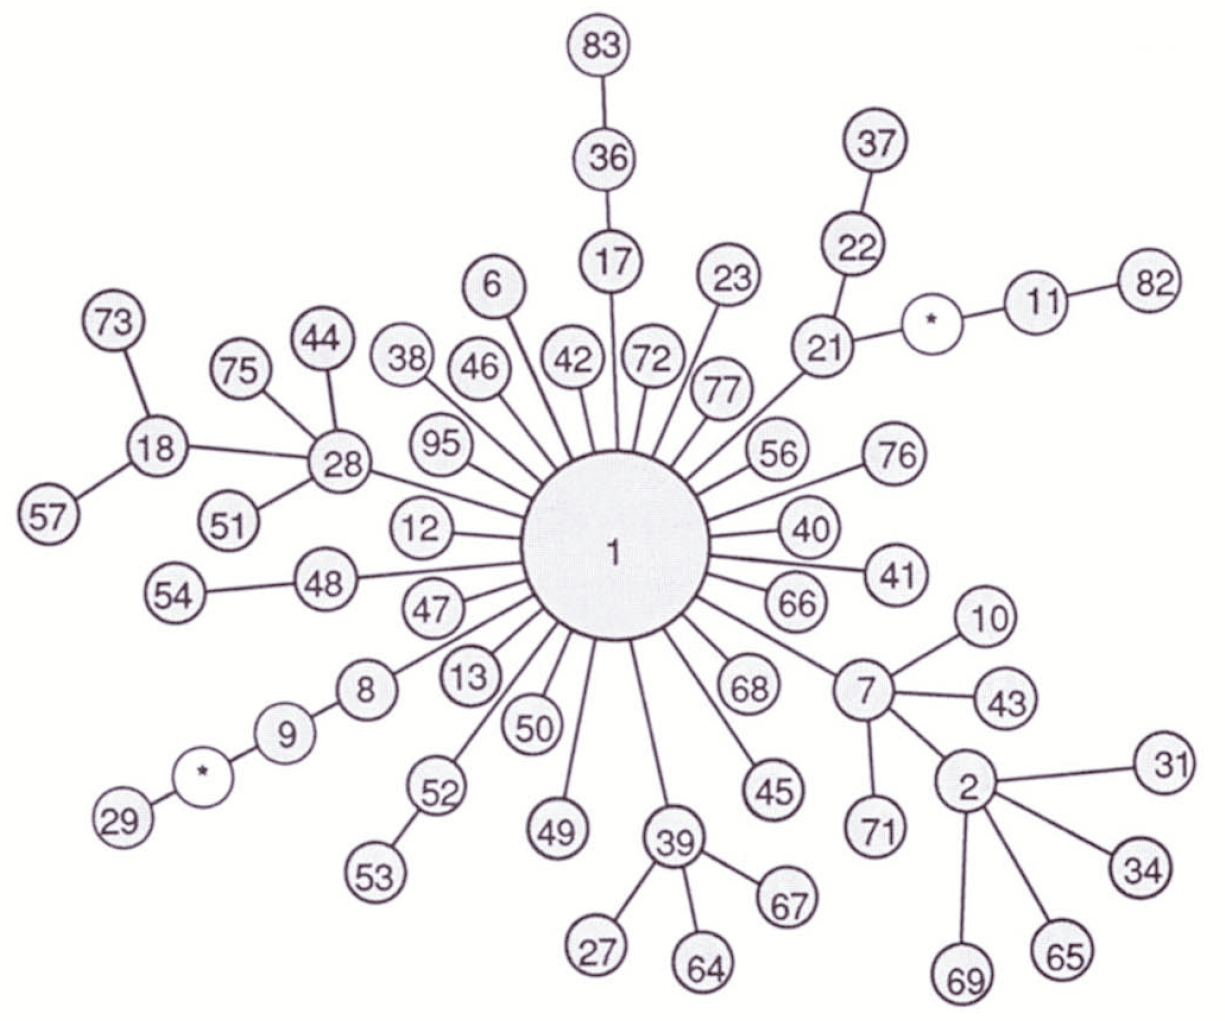
\includegraphics{amova-haplotypes.eps}}
\end{center}
}

\myslide{
\begin{center}
\begin{tabular}{lc}
\hline\hline
Component of differentiation     & $\Phi$-statistics \\
\hline
Among regions                    & $\Phi_{CT} = 0.220$ \\
Among populations within regions & $\Phi_{SC} = 0.044$ \\
Among all populations            & $\Phi_{ST} = 0.246$ \\
\hline
\end{tabular}
\end{center}
}

\myslide{
\begin{center}
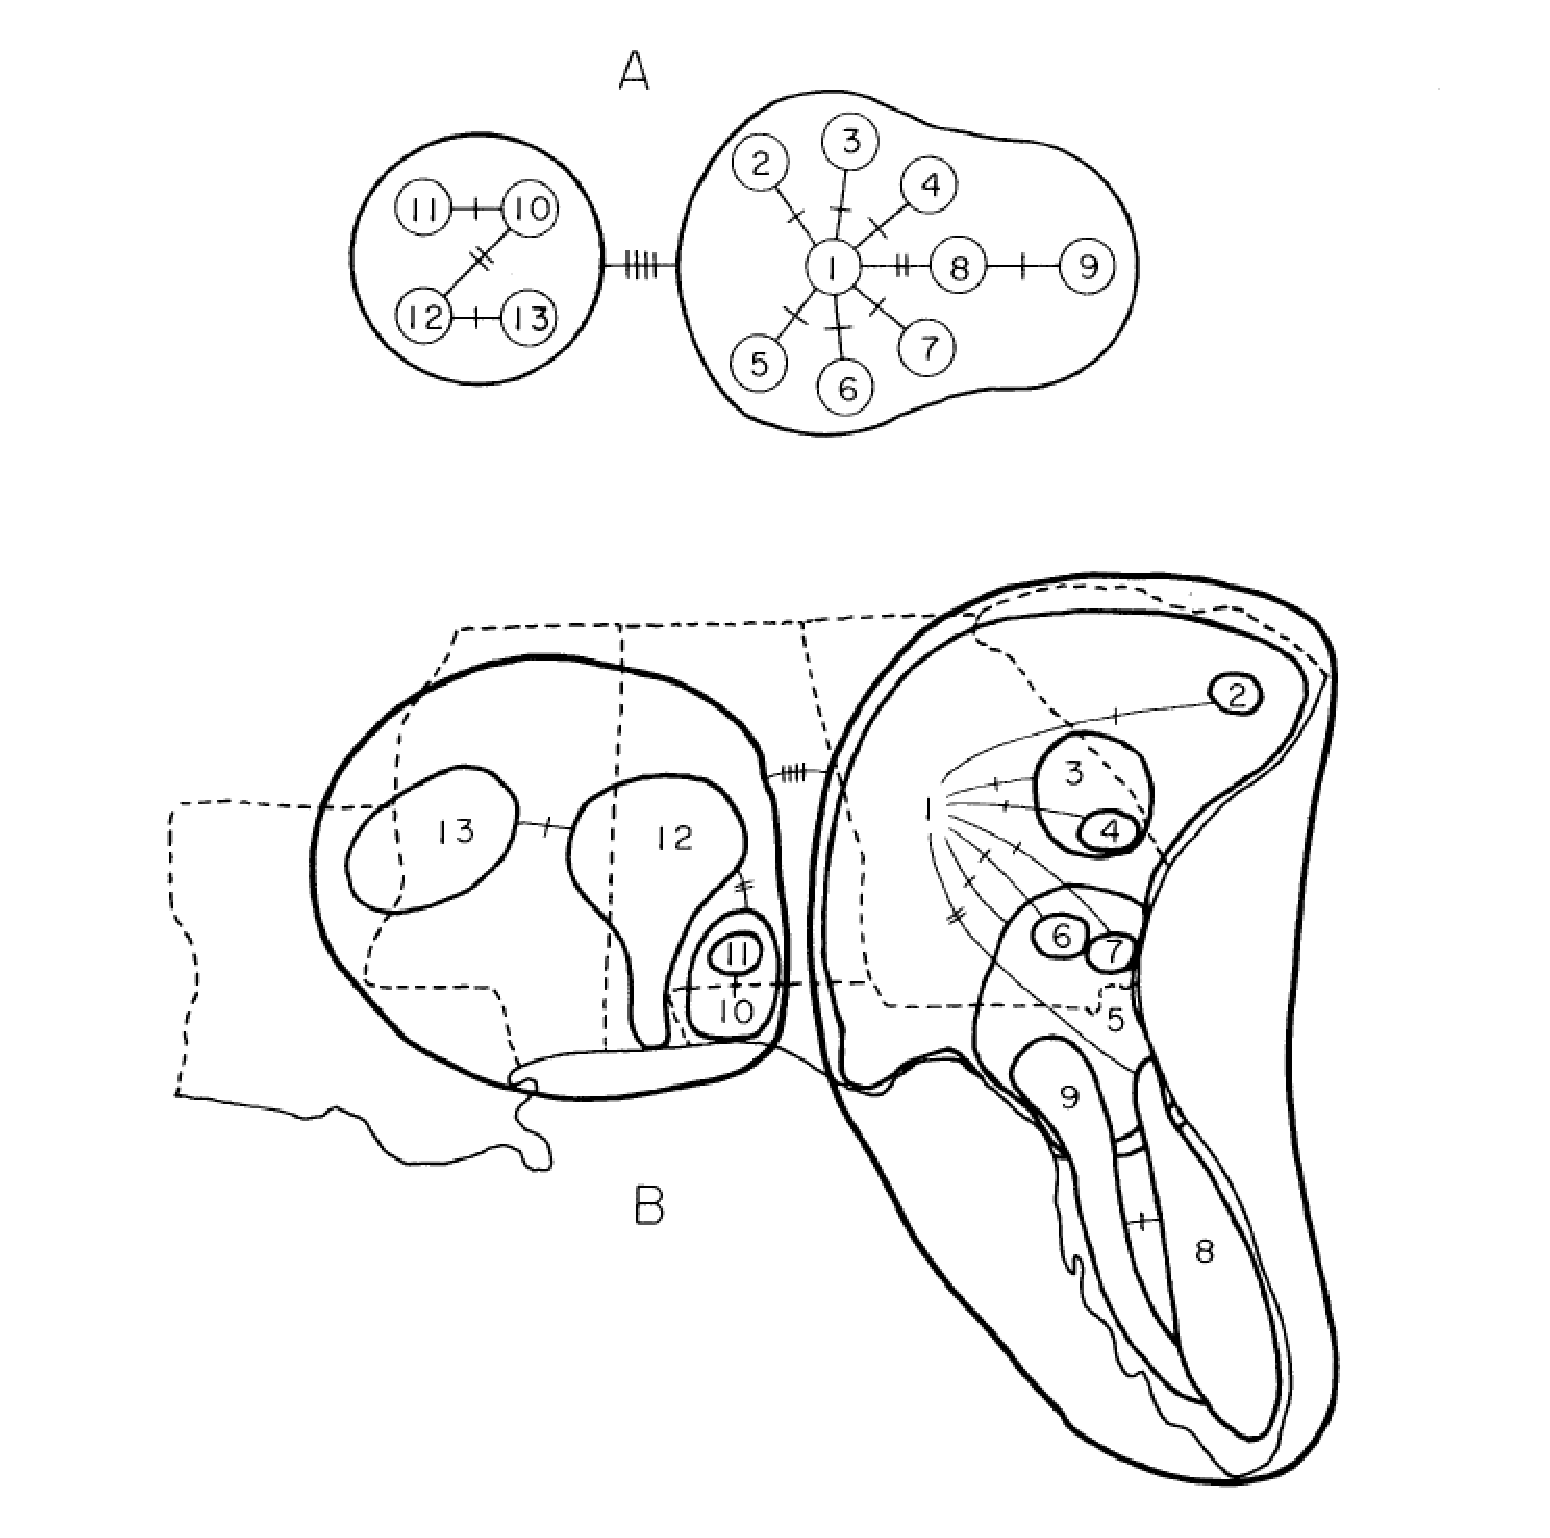
\includegraphics[width=0.75\textwidth]{bowfin-phylogeography.eps}
\end{center}
}

\myslide{
\begin{center}
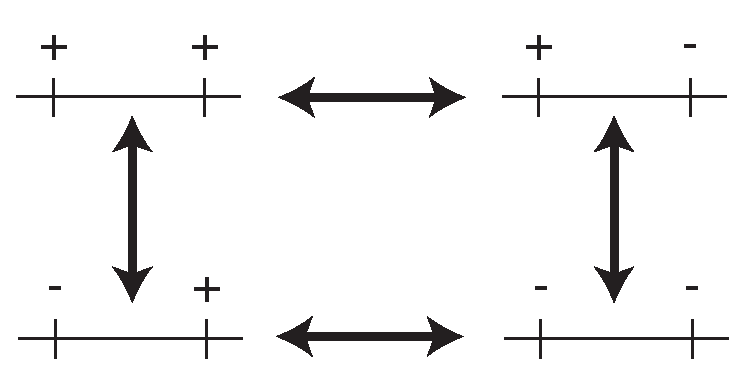
\includegraphics[width=0.75\textwidth]{haplotype-network.eps}
\end{center}
}

\myslide{
\begin{center}
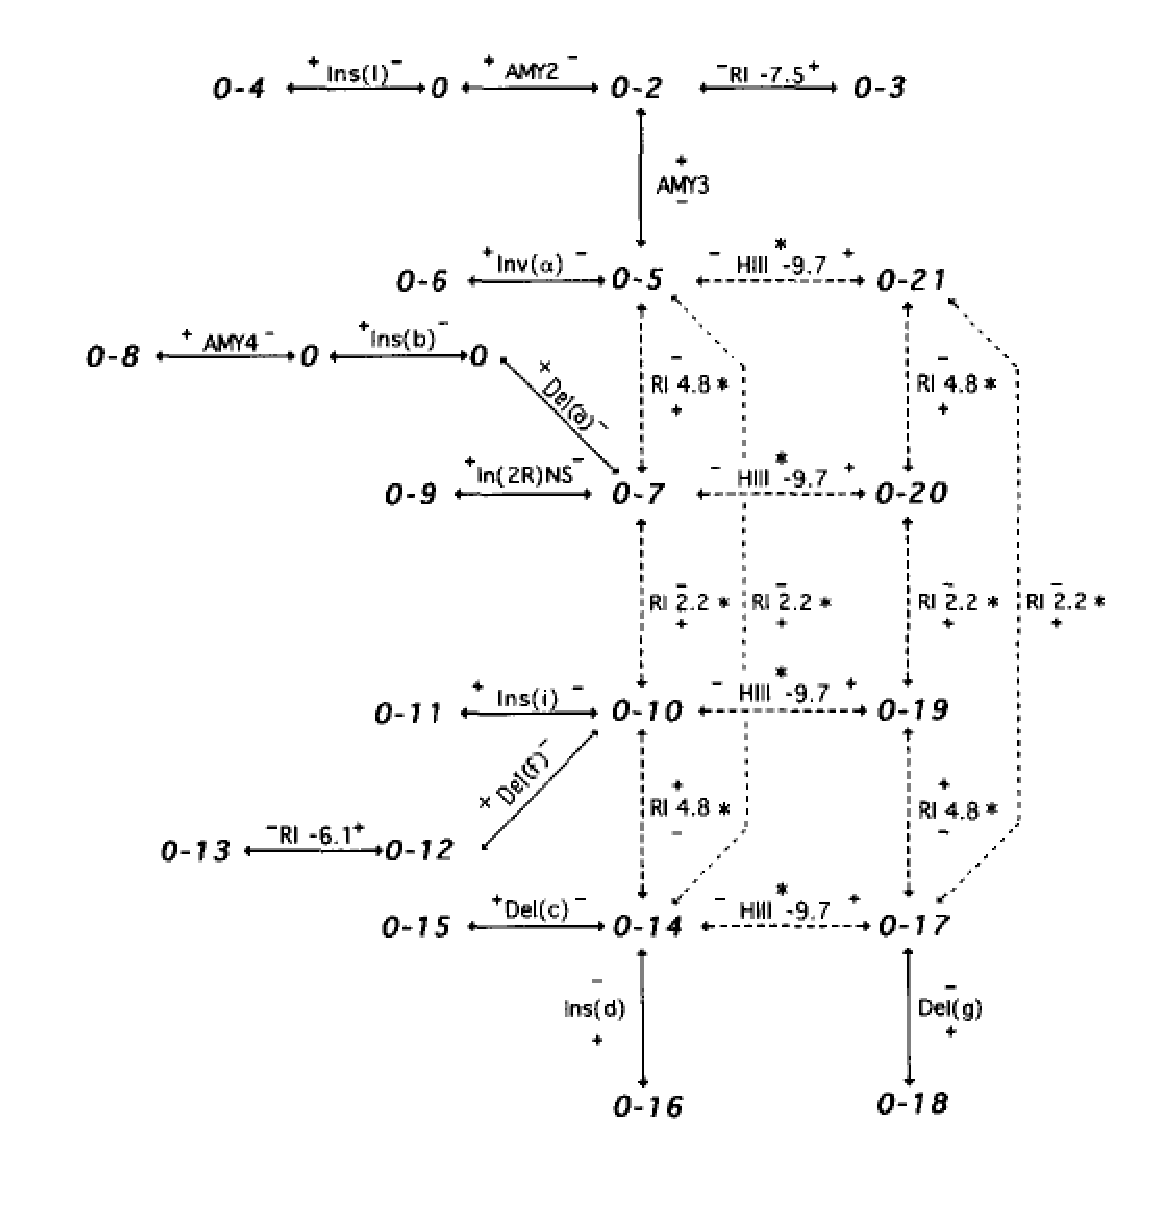
\includegraphics[width=0.7\textwidth]{amy-tcs.eps}
\end{center}
}

\myslide{
\begin{center}
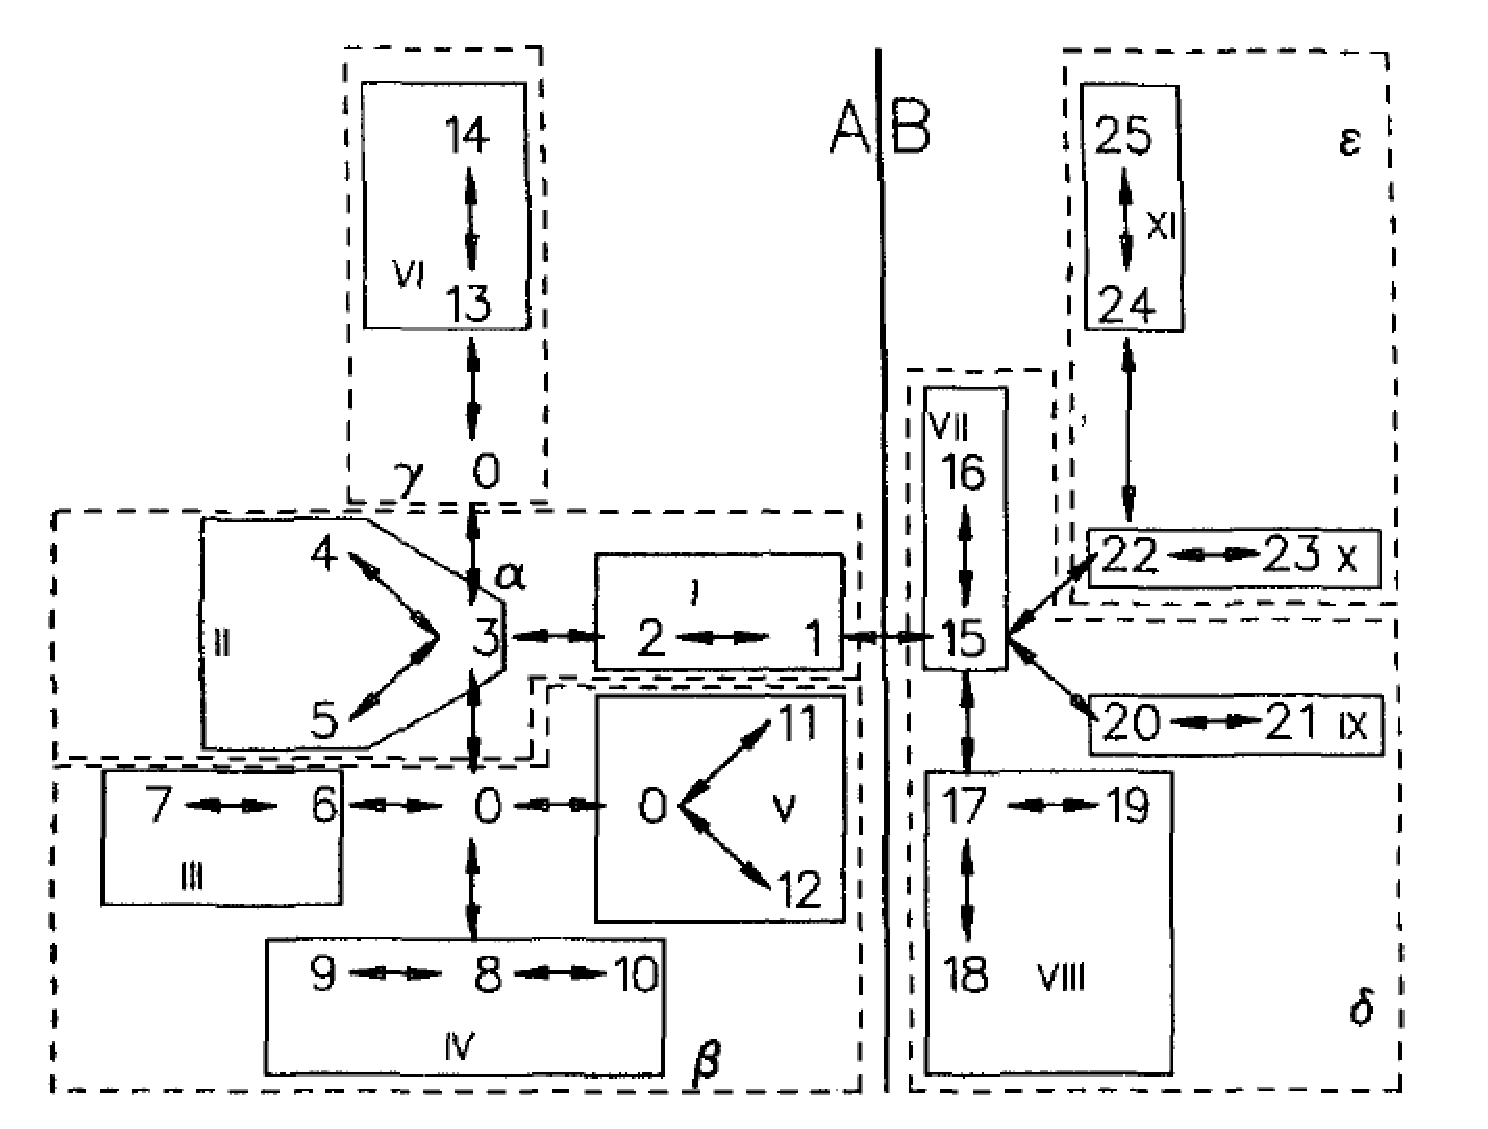
\includegraphics[width=0.75\textwidth]{nca-nesting.eps}
\end{center}
}

\myslide{
\begin{center}
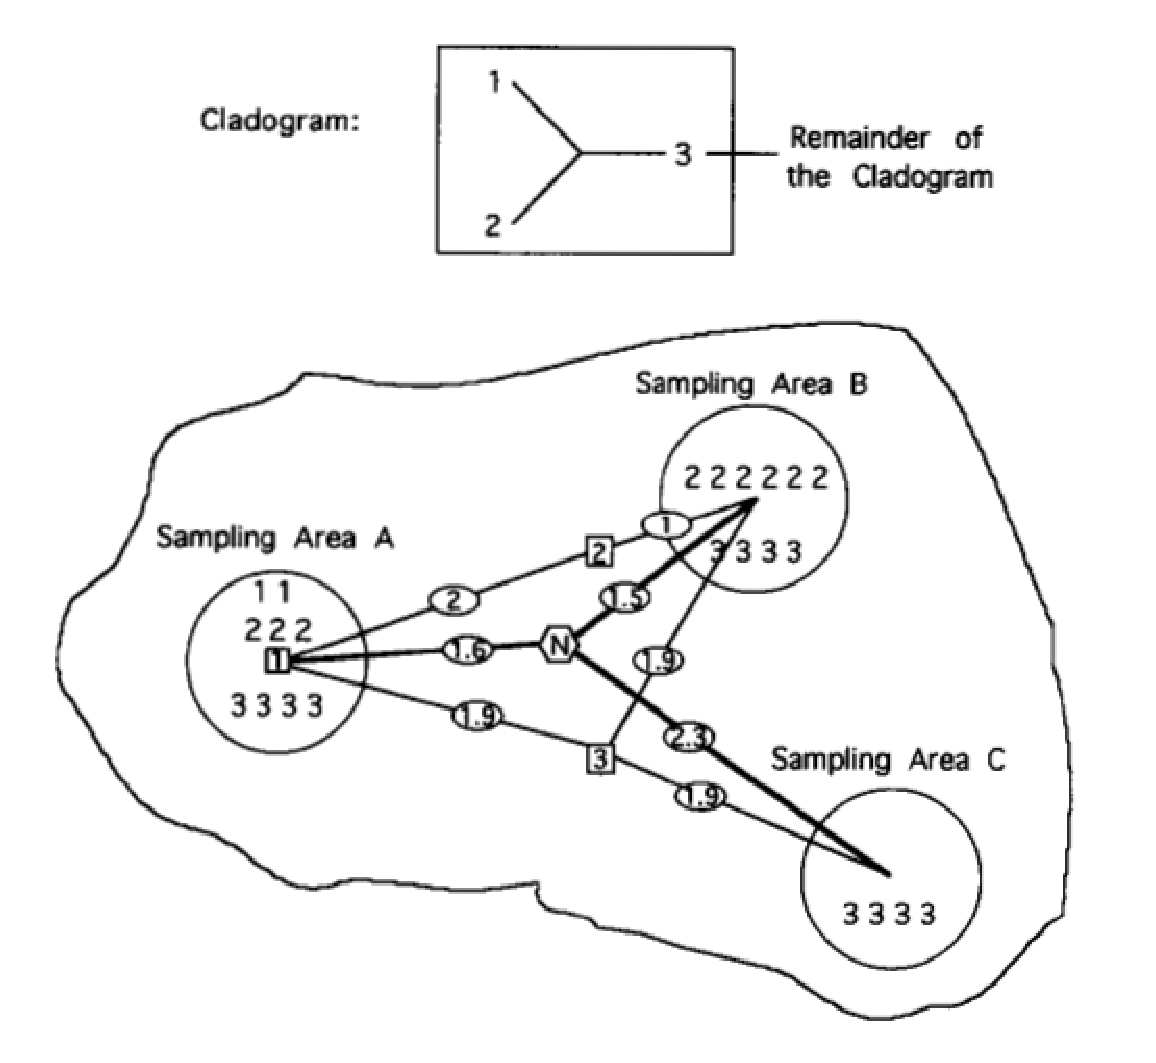
\includegraphics[width=0.75\textwidth]{nca-calculations.eps}
\end{center}
}

\myslide{
\begin{center}
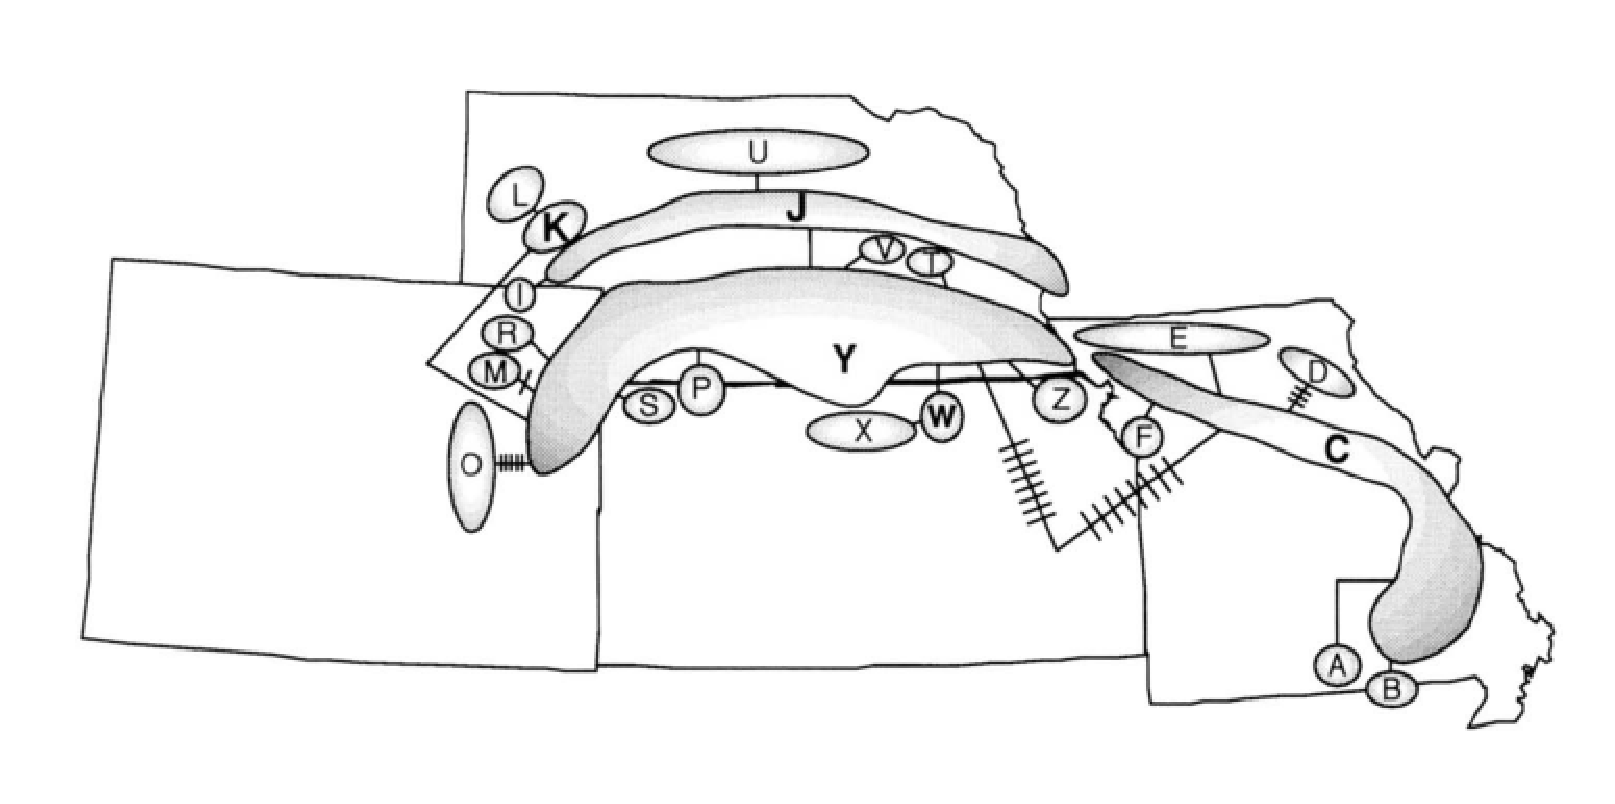
\includegraphics[width=0.75\textwidth]{ambystoma.eps}
\end{center}
}

\myslide{
\begin{center}
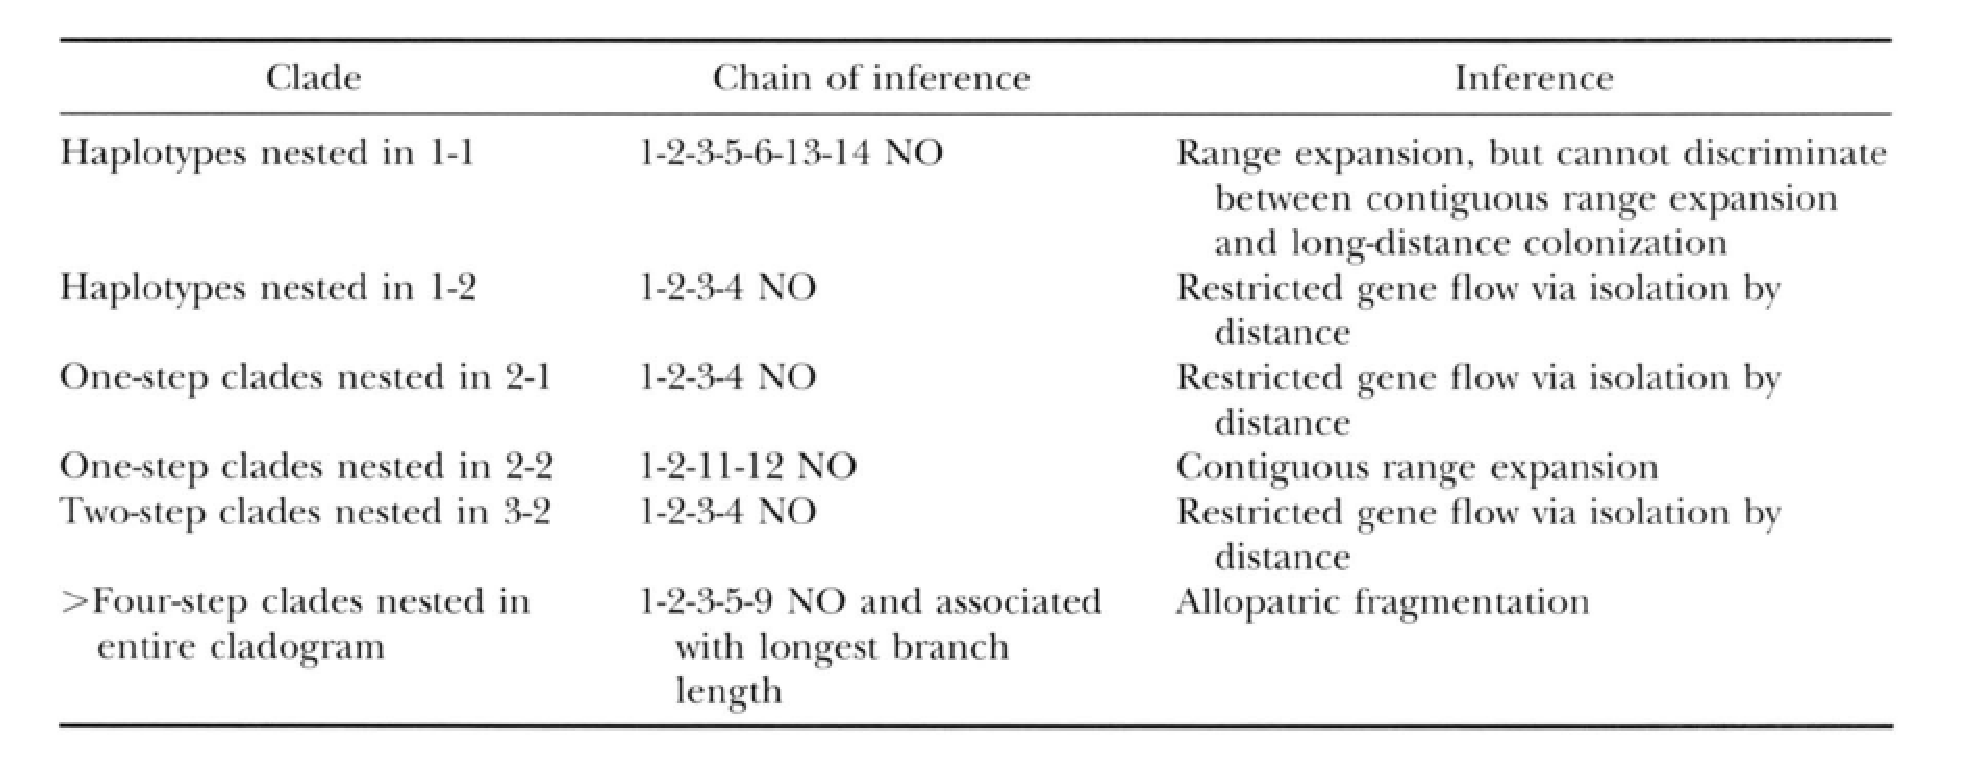
\includegraphics[width=\textwidth]{ambystoma-inference.eps}
\end{center}
}

\myslide{
\begin{center}
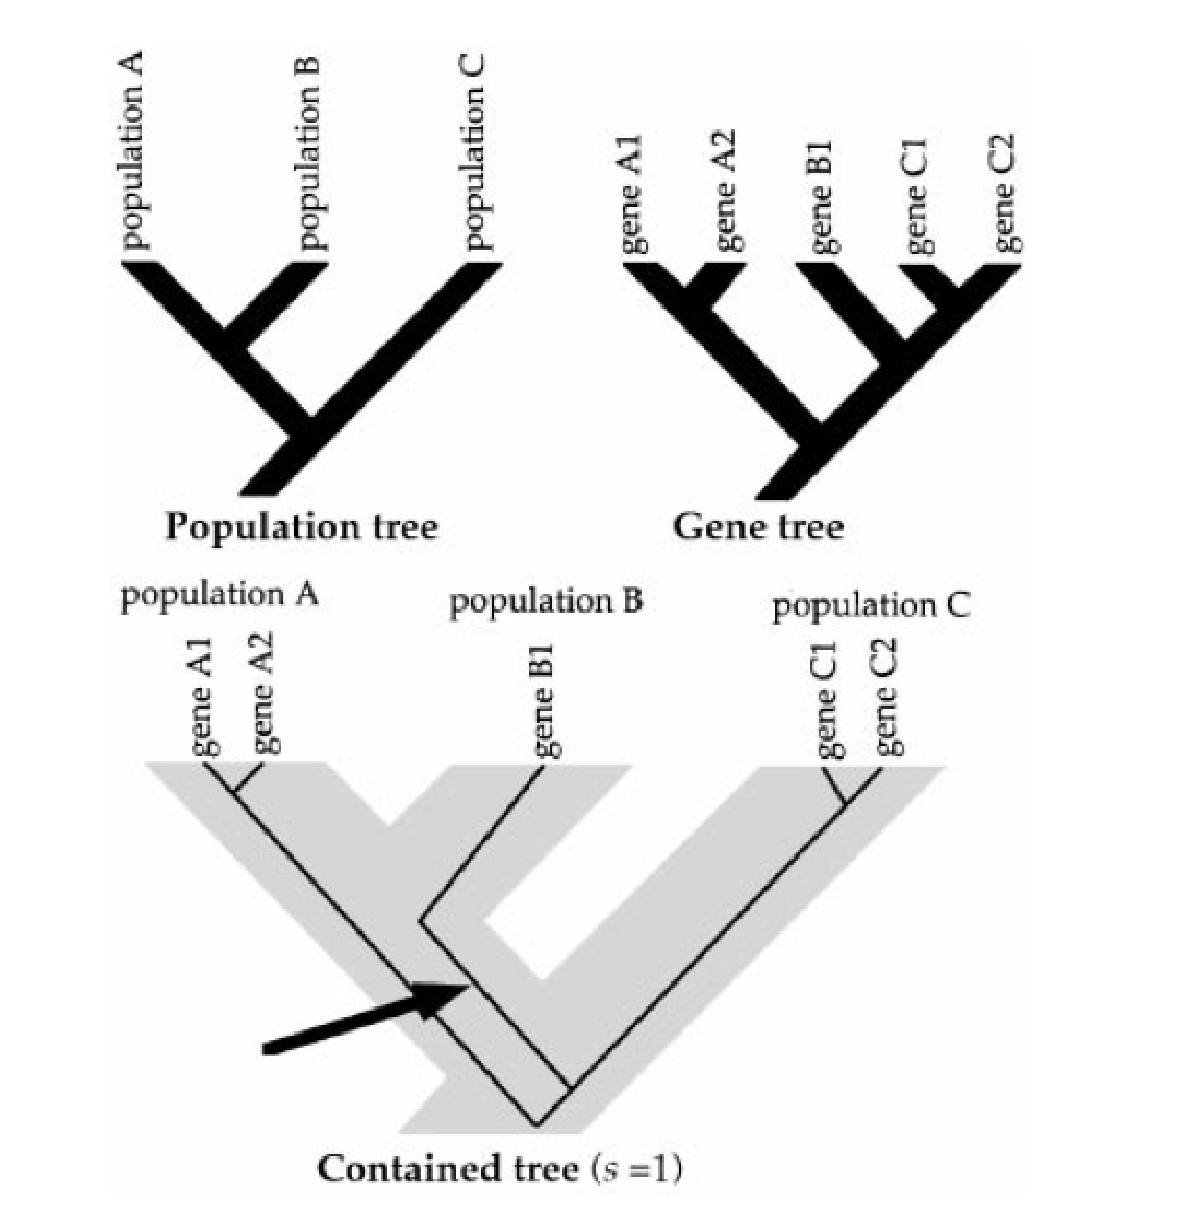
\includegraphics[width=0.7\textwidth]{ancestral-polymorphism.eps}
\end{center}
}

\myslide{
\begin{center}
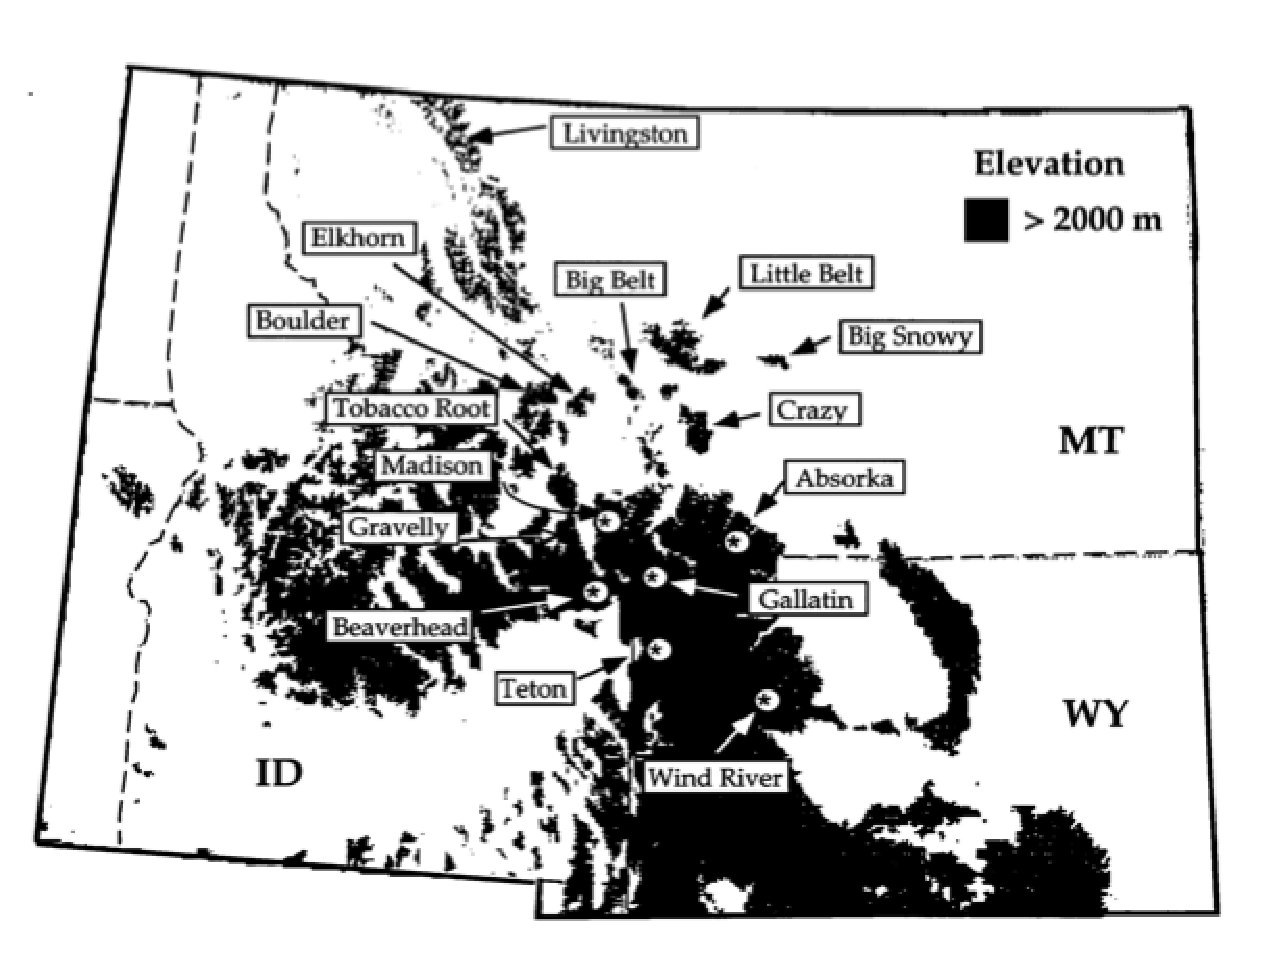
\includegraphics[height=6cm]{sky-islands.eps}
\end{center}
}

\myslide{
\begin{center}
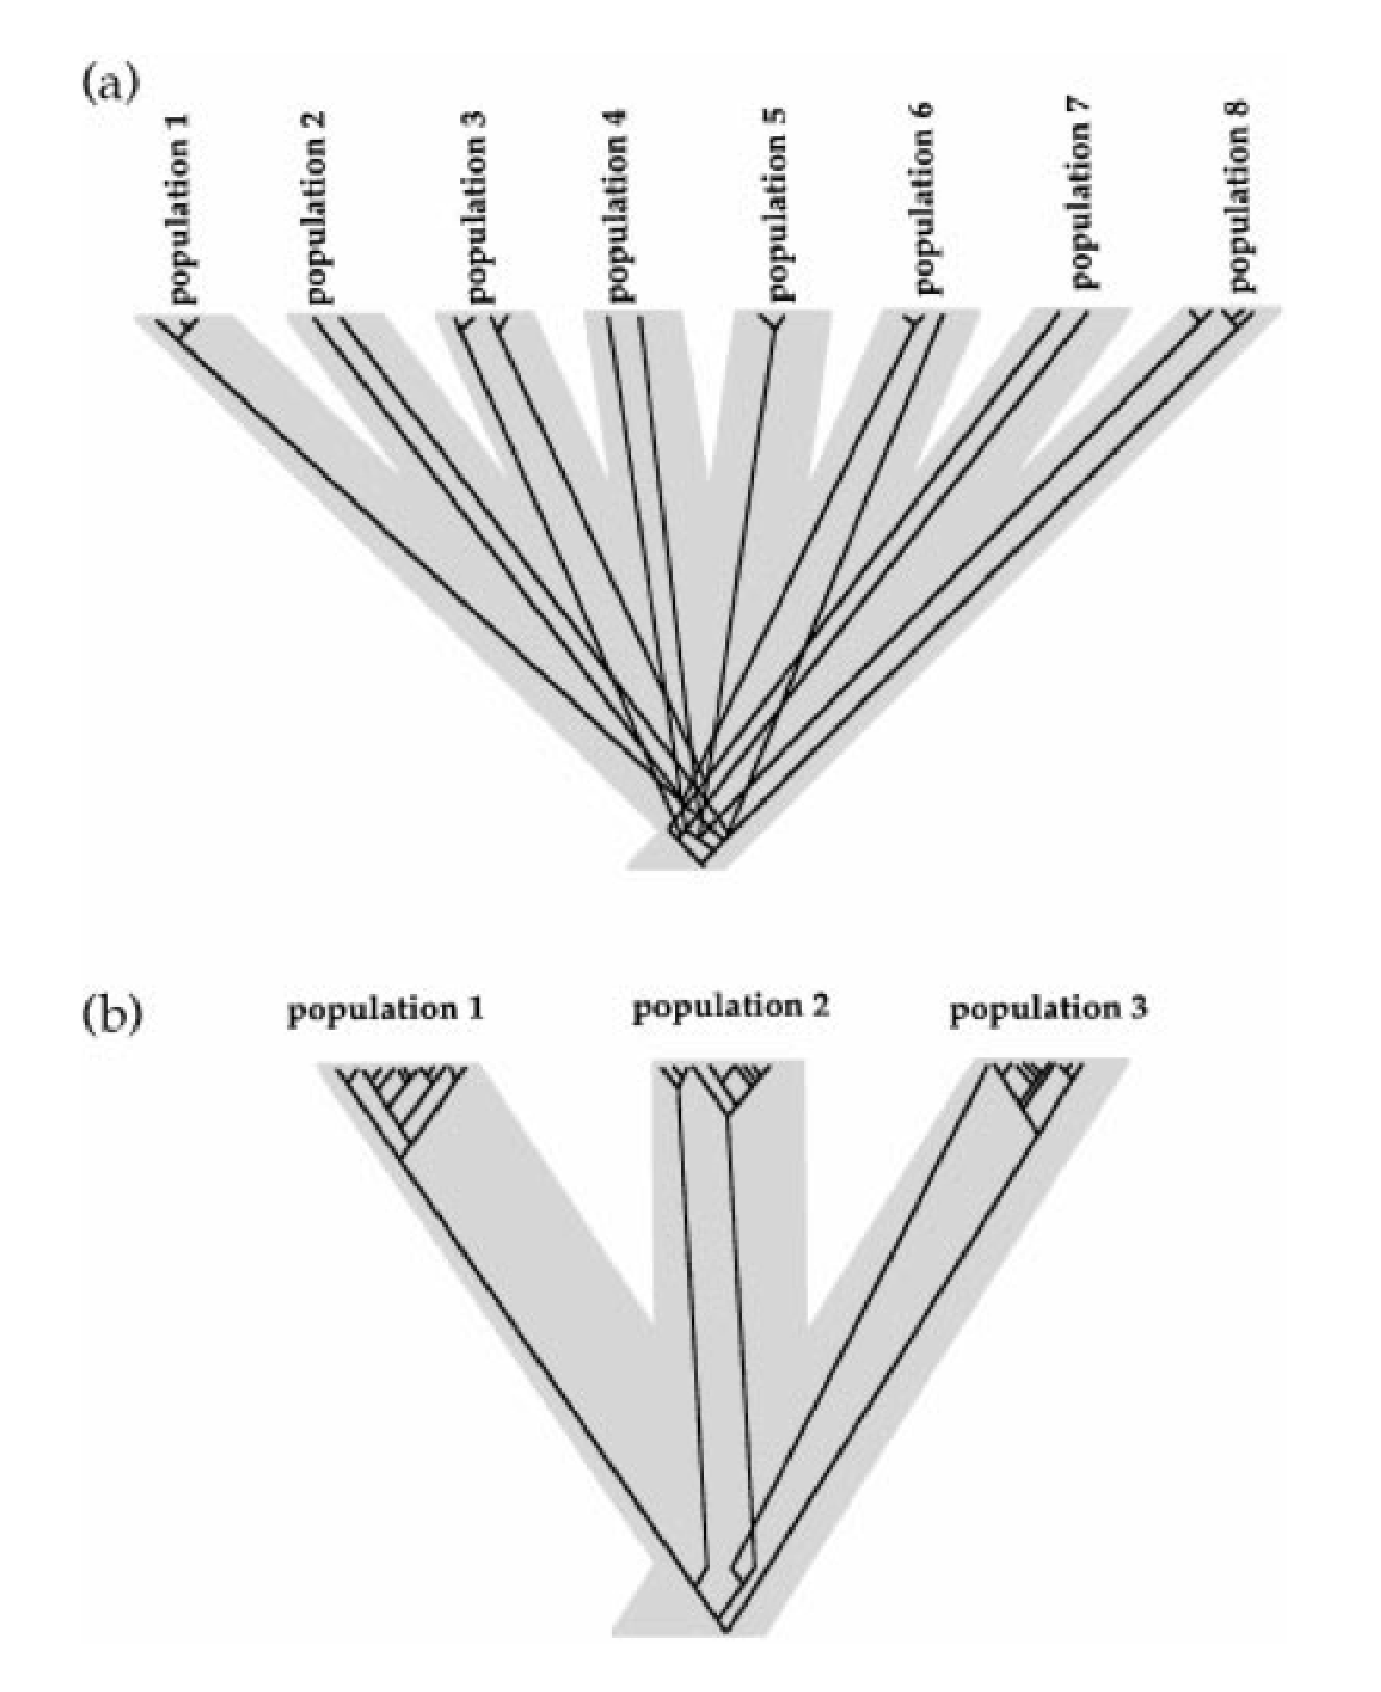
\includegraphics[height=6cm]{divergence-hypotheses.eps}
\end{center}
}

\end{document}


